% =============================================================================
% Greeks Engine -- IEEE conference paper (IEEEtran, conference mode).
% Build: pdflatex greeks_engine_ieee.tex (twice). Figures: make_paper_figures.py.
% CPU energy: validation/cpu_baseline/cpu_energy.py (HWiNFO session, 29 Oct 2026).
% =============================================================================
\documentclass[conference]{IEEEtran}
\IEEEoverridecommandlockouts
\usepackage{cite}
\usepackage{amsmath,amssymb}
\usepackage{graphicx}
\usepackage{booktabs}
\usepackage{multirow}
\usepackage{array}
\newcolumntype{L}[1]{>{\raggedright\arraybackslash}p{#1}}
\usepackage{xcolor}
\usepackage{url}
\usepackage{tikz}
\usetikzlibrary{arrows.meta,positioning,fit,calc,backgrounds}
\usepackage[hidelinks]{hyperref}

\newcommand{\TBD}[1]{\textcolor{red}{\textbf{[#1]}}}
% vectorised CPU baseline (validation/cpu_baseline/run_simd.py -> results/cpu_simd.csv)
\newcommand{\SIMDUS}{13.6}
\newcommand{\SIMDTP}{216,000}
\definecolor{acc}{HTML}{0072B2}
\definecolor{accsoft}{HTML}{DCEBF5}
\definecolor{ink}{HTML}{16202A}
\definecolor{muted}{HTML}{56626B}
\tikzset{
  blk/.style={draw=ink, fill=white, rounded corners=1.5pt, align=center, font=\scriptsize, inner sep=2.5pt, minimum height=0.75cm},
  key/.style={blk, fill=accsoft, draw=acc, font=\scriptsize\bfseries},
  arr/.style={-{Stealth[length=1.6mm]}, semithick, draw=ink},
  darr/.style={-{Stealth[length=1.6mm]}, semithick, draw=muted, dashed},
  lbl/.style={font=\tiny, text=muted, align=center},
}

\begin{document}

\title{Co-Scheduled Adjoint Greeks in a Fixed-Point FPGA Datapath:\\ Heston-Model Option Sensitivities with First-Order Rounding Bounds}

\author{\IEEEauthorblockN{Yash Agrawal}
\IEEEauthorblockA{Birla Institute of Technology and Science, Pilani\\ Pilani, India}
\and
\IEEEauthorblockN{Govind Prasad}
\IEEEauthorblockA{Birla Institute of Technology and Science, Pilani\\ Pilani, India}}

\maketitle
\begin{abstract}
FPGA option-pricing engines obtain Greeks, the sensitivities of a price to its inputs, by
bump-and-reprice or by re-simulation. We present an FPGA engine for European options under the
Heston model, priced with the COS Fourier-cosine method, in which a hand-derived reverse (adjoint)
sweep is co-scheduled with the forward pass in one statically scheduled fixed-point datapath.
Because the COS loop has no data-dependent control flow, the values the reverse sweep needs are
held in a statically allocated, register-resident tape rather than in memory. A generator emits,
from one operation graph, a bit-accurate model, the modulo-scheduled Verilog and a first-order
rounding-error bound for the price and each of nine first-order Greeks, used at design time to
size and certify the word length. Implemented in Vivado on a Zynq-7020 at equal throughput, the
price-and-Greeks engine takes 1.03$\times$ the cycles of a price-only engine at 1.68$\times$ its
LUTs and 2$\times$ its DSP blocks; a factored forward-mode engine built by the same flow needs 7\%
more LUTs, 12\% more flip-flops and 25\% more DSP blocks and is 6$\times$ less accurate at the same
word length. The bound was never exceeded over 21,000 inputs, and the engine ran bit-exact on two
FPGA families (1,469/1,469 outputs, including 50 calibrations to NIFTY options). The bound covers
rounding only; the COS truncation error dominates in a few in-domain cases. The computed engine
latency on a ZCU102, 15.9\,$\mu$s excluding bus transfers, is 4.9--15$\times$ below
general-purpose AD and bump-and-reprice on a laptop core but not below a vectorised implementation
of hand-derived Greeks (\SIMDUS\,$\mu$s).
\end{abstract}

\begin{IEEEkeywords}
FPGA, adjoint differentiation, option Greeks, Heston model, COS method, fixed-point arithmetic,
rounding-error analysis, modulo scheduling
\end{IEEEkeywords}

% =============================================================================
\section{Introduction}
Option Greeks, the partial derivatives of a price with respect to spot, strike, maturity, rate
and the model's parameters, set hedge ratios and risk limits and drive model calibration. Under
the Heston model~\cite{heston} the price has no closed form and is computed numerically, here by
the COS method~\cite{fang}. Published FPGA engines compute Greeks by bump-and-reprice or by
re-simulation~\cite{klai,klaih2rc,vitisquant}: nine Greeks by central differences cost 19
pricings, with an accuracy that depends on a bump size no setting of which suits every Greek
(Fig.~\ref{fig:bump}). Software uses adjoint algorithmic differentiation (AAD)~\cite{giles,capriotti,capgiles24},
which returns all derivatives of one output in a single reverse sweep but records a tape of the
forward computation; our taped CPU baseline costs 7.6 pricings.

A reverse sweep over code without data-dependent control flow can be scheduled statically, as in
source-transformation AD~\cite{tapenade} and neural-network training accelerators. The COS pricer
has this property: each of its 128 terms runs the same operations. We co-schedule a hand-derived
reverse sweep with the forward pass in one fixed-point datapath and measure what the Greeks cost
in time, area and accuracy against alternatives built through the same flow. Contributions:
\begin{enumerate}
\item \textbf{A co-scheduled adjoint datapath} for Heston--COS Greeks with a statically allocated,
register-resident tape (Section~\ref{sec:method}). After a literature search
(Section~\ref{sec:background}) we know of no prior FPGA computation of Greeks by an adjoint and no
prior FPGA COS implementation.
\item \textbf{A measured cost of the Greeks}: price-only, adjoint and factored forward-mode engines
of equal throughput implemented in Vivado through the same flow (Section~\ref{sec:res-cost}).
\item \textbf{A first-order rounding-error bound for every Greek} of a datapath that contains its own
reverse sweep, extending AD-based precision analysis for FPGAs~\cite{gaffar,lee06}, with its scope
and the modelling of the primitives stated (Sections~\ref{sec:bound},~\ref{sec:res-acc}).
\item \textbf{A generator and bit-exact silicon results} on two FPGA families, including
calibrations to market data (Section~\ref{sec:res-silicon}).
\end{enumerate}
Not claimed: an AD tool (the reverse sweep is derived by hand); a bound attached to each result
(it is computed at design time and covers rounding only); speed or energy advantages over a
vectorised CPU (Section~\ref{sec:res-cpu}).

% =============================================================================
\section{Background and Related Work}
\label{sec:background}
\textbf{Heston and COS.} The Heston model has $\mathrm{d}S_t = rS_t\,\mathrm{d}t + \sqrt{v_t}S_t\,\mathrm{d}W_1$,
$\mathrm{d}v_t = \kappa(\theta-v_t)\,\mathrm{d}t + \xi\sqrt{v_t}\,\mathrm{d}W_2$,
$\mathrm{d}W_1\mathrm{d}W_2=\rho\,\mathrm{d}t$ and nine pricing inputs
$p=(S_0,K,T,r,v_0,\kappa,\theta,\xi,\rho)$; we use the characteristic function $\varphi$ in the
form of Albrecher et al.~\cite{albrecher}. The COS method~\cite{fang} expands the density on a
truncation range $[a,b]$ in a cosine series; for a put
\begin{equation}
V_{\mathrm{put}} \approx K e^{-rT}\,{\sum_{k=0}^{N-1}}{}^{\prime}\,
\mathrm{Re}\!\left[\varphi(u_k)\,e^{\,iu_k(x-a)}\right] U_k,\quad u_k=\tfrac{k\pi}{b-a},
\label{eq:cos}
\end{equation}
with $x=\ln(S_0/K)$ and closed-form payoff coefficients $U_k$; calls follow from put--call parity,
and the $N$ terms are independent. Delta and Gamma have closed-form COS
expressions~\cite[Remark~3.2]{fang},~\cite{junike}, and $\partial V/\partial K$ follows from Delta, so these
are nearly free in any COS implementation; the derivatives in $T$, $r$ and the five model parameters
enter through $\varphi$, and these are where differentiation does real work.

\textbf{Greeks.} Bump-and-reprice has truncation error $O(h^2)$ and rounding error
$O(\epsilon/h)$. Forward-mode AD carries a tangent per input; reverse-mode AD returns all
derivatives in one sweep at a small multiple of the pricing cost~\cite{griewank}, storing forward
values on a tape or recomputing them under checkpointing~\cite{griewank92}. Cui et
al.~\cite{cui} derived the Heston--Fourier gradient by hand.

\textbf{Hardware.} FPGA option pricing covers Heston Monte Carlo~\cite{deschryver,deschryver13},
trees~\cite{jin} and quadrature~\cite{tse}; the STAC-A2 risk benchmark, with Greeks by
re-simulation, has been ported to Alveo, Stratix-10 and Versal devices~\cite{klai,klaih2rc,klai24},
and AMD's library computes Greeks by central differences~\cite{vitisquant}. COS pricing has been
accelerated on GPUs, including Heston and many strikes~\cite{zhang09,zhang14}, and adjoint AD runs on
GPUs with a tape~\cite{gremse}. Table~\ref{tab:related} summarises. We found no FPGA adjoint Greeks
and no FPGA COS implementation in FPL, FCCM, FPT, ReConFig, TRETS, HEART, H2RC and general indexes;
absence from a search is not proof of absence.

\textbf{Precision analysis.} AD-based word-length analysis for FPGAs goes back to Gaffar et
al.~\cite{gaffar}, accuracy-guaranteed bit-width optimisation to Lee et al.~\cite{lee06}, and
Gappa~\cite{gappa} gives machine-checked enclosures. Our bound is Linnainmaa's first-order
analysis~\cite{linnainmaa} applied to a datapath that contains its own adjoint; we do not compare
its tightness with affine-arithmetic or Gappa enclosures.

\begin{table}[!t]
\centering
\caption{Related work (figures not directly comparable)}
\label{tab:related}
\footnotesize
\setlength{\tabcolsep}{2.5pt}
\begin{tabular}{@{}L{2.2cm}L{1.5cm}L{2.0cm}L{2.5cm}@{}}
\toprule
\textbf{Work} & \textbf{Platform} & \textbf{Pricing} & \textbf{Greeks by}\\
\midrule
\cite{deschryver,deschryver13} & FPGA & Heston MC & --- (price only)\\
\cite{jin,tse} & FPGA & trees, quadrature & ---\\
\cite{klai,klaih2rc,klai24} & FPGA, ACAP & STAC-A2 (Heston MC) & re-simulation\\
\cite{vitisquant} & FPGA (HLS) & Heston MC & central differences\\
\cite{zhang09,zhang14} & GPU & COS & --- (price only)\\
\cite{gremse} & GPU & general & taped adjoint AD\\
\cite{cui} & CPU & Heston, Fourier & analytic (by hand)\\
\midrule
\textbf{This work} & FPGA & Heston, COS & \textbf{co-scheduled adjoint, per-Greek rounding bound}\\
\bottomrule
\end{tabular}
\end{table}

% =============================================================================
\section{Method}
\label{sec:method}
\textbf{A register-resident tape.} A reverse sweep needs the forward values in reverse order. In
(\ref{eq:cos}) every term runs the same operations, the range is fixed per evaluation, and nothing
branches on data, so the forward and reverse operations of one term form a fixed graph whose every
value has a lifetime known at design time. The modulo scheduler allocates each value the rotating
registers that hold it across the terms in flight: the tape costs registers, not memory traffic.
Over all terms in flight the 56-bit adjoint datapath needs 447 such registers, against 150 for a
price-only datapath of equal throughput and 374 for the factored forward one. The Greeks are
derivatives of the COS approximation with $[a,b]$ held fixed (A4, Table~\ref{tab:assumptions});
per term the sweep propagates adjoints to the model inputs, reusing the forward reciprocals, a
power-of-two normalisation keeps small adjoints at full precision, and nine accumulators sum the
results.

\textbf{Arithmetic.} No dividers: reciprocals and square roots use Newton--Raphson from table seeds,
the exponential Tang's method~\cite{tang}, the logarithm a table and series, and sines, cosines and
complex magnitudes and angles CORDIC~\cite{volder}. A term costs 250 multiplications, three CORDIC
rotations and two vectorings (126 multiplications for the price alone). Values are fixed point with
$FL$ fraction bits (56-bit words with $FL=28$, or 64 with $FL=32$), rounded to nearest after every
operation; shifters are built only as wide as the ranges measured over the domain, and an input
beyond a range raises \texttt{range\_err}.

\textbf{First-order rounding-error bound.}
\label{sec:bound}
With local errors $|\delta_i|\le\epsilon_i$ at operations $w_i$, to first order
\begin{equation}
|\hat y - y| \;\le\; \sum_i \left|\partial y/\partial w_i\right| \epsilon_i =: B_y ,
\label{eq:bound}
\end{equation}
Linnainmaa's analysis~\cite{linnainmaa}; the sensitivities come from a reverse sweep over the graph,
which includes the hardware's own adjoint operations, so $B_y$ bounds the rounding error of each
Greek as computed. $B_y$ bounds the difference from the \emph{same graph} in exact arithmetic. The
primitives are expanded into graph operations (Newton--Raphson steps, table lookups, series terms),
each with $\epsilon_i = 2^{-(FL+1)}$; their approximation error is common to both evaluations and
measured separately ($\le1.1\times10^{-8}$ relative against exact functions). Each CORDIC unit is one
operation whose error was measured against its exact integer model over 30,000 inputs: rotation
within 1.14\,ulp (modelled as 2\,ulp); vectoring magnitude within 0.8\,ulp; the vectoring angle
within $1.75/|z|$\,ulp, modelled as $2\max(1,1/|z|)$\,ulp. The COS truncation error is excluded
(Section~\ref{sec:res-acc}). $B_y$ takes 0.1\,s per input in software, so it is a design-time tool
for choosing and certifying the word length (Table~\ref{tab:acc}), not attached to each result.

\textbf{Generator and schedule.} One Python description of setup, term ($N=128$) and finish is an
operation graph from which the generator derives the bit-accurate model, a double-precision model,
the bound and a modulo schedule~\cite{rau} emitted as Verilog (Fig.~\ref{fig:flow}); the testbench
compares every register against the model at the cycle it becomes valid. A new term starts every
initiation interval (II, Fig.~\ref{fig:sched}); with 8 multipliers, 3 CORDIC rotators and 2 vectorers
all three resources give $\mathrm{II}=\lceil 250/8\rceil=32$, and the loop takes $127\cdot32+506+2=4{,}572$
cycles. The reverse sweep's extra 124 multiplications per term fit into multiplier slots the
CORDIC-bound forward pass leaves idle, but only because the engine has twice the multipliers a
price-only engine needs for the same II ($\lceil126/32\rceil=4$).

\begin{figure*}[!t]
\centering
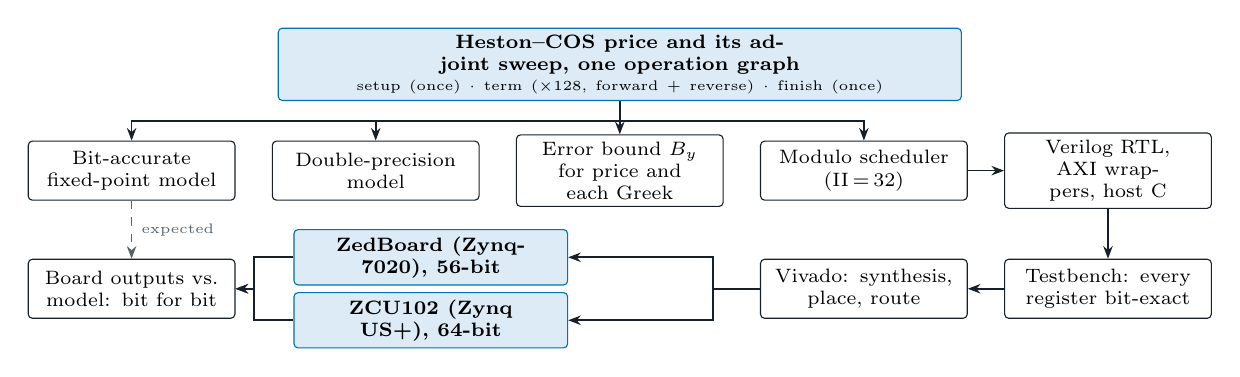
\begin{tikzpicture}[node distance=0.35cm]
  \node[key, text width=8.5cm] (src) at (0,0) {Heston--COS price and its adjoint sweep, one operation graph\\[-1pt]
    \normalfont\tiny setup (once) $\cdot$ term ($\times$128, forward + reverse) $\cdot$ finish (once)};
  \foreach \x/\n/\t in {-6.2/emu/{Bit-accurate\\fixed-point model}, -3.1/flt/{Double-precision\\model},
                        0/bnd/{Error bound $B_y$\\for price and each Greek}, 3.1/sch/{Modulo scheduler\\(II\,=\,32)}, 6.2/rtl/{Verilog RTL,\\AXI wrappers, host C}}
    \node[blk, text width=2.45cm] (\n) at (\x,-1.35) {\t};
  \foreach \n in {emu,flt,bnd,sch} \draw[arr] (src.south) -- ++(0,-0.25) -| (\n.north);
  \draw[arr] (sch) -- (rtl);
  \node[blk, text width=2.45cm] (tb) at (6.2,-2.85) {Testbench: every\\register bit-exact};
  \node[blk, text width=2.45cm] (viv) at (3.1,-2.85) {Vivado: synthesis,\\place, route};
  \node[key, text width=3.3cm, minimum height=0.55cm] (zed) at (-2.4,-2.45) {ZedBoard (Zynq-7020), 56-bit};
  \node[key, text width=3.3cm, minimum height=0.55cm] (zcu) at (-2.4,-3.25) {ZCU102 (Zynq US+), 64-bit};
  \node[blk, text width=2.45cm] (cmp) at (-6.2,-2.85) {Board outputs vs.\\model: bit for bit};
  \draw[arr] (rtl) -- (tb); \draw[arr] (tb) -- (viv);
  \draw[arr] (viv.west) -- ++(-0.6,0) |- (zed.east); \draw[arr] (viv.west) -- ++(-0.6,0) |- (zcu.east);
  \draw[arr] (zed.west) -- ++(-0.5,0) |- (cmp.east); \draw[arr] (zcu.west) -- ++(-0.5,0) |- (cmp.east);
  \draw[darr] (emu) -- node[lbl, right] {expected} (cmp);
\end{tikzpicture}
\caption{Design flow. One operation graph yields the bit-accurate model, the error bound and the scheduled RTL; the RTL is checked register by register against the model, implemented in Vivado and run on two boards, whose outputs are compared bit for bit with the same model.}
\label{fig:flow}
\end{figure*}

\begin{figure}[!t]
\centering
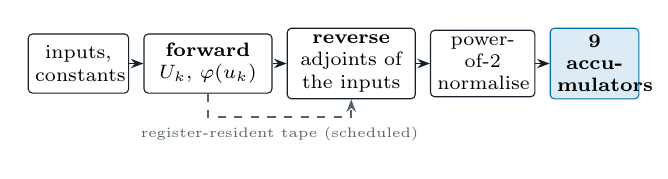
\begin{tikzpicture}[node distance=0.18cm]
  \node[blk, text width=1.1cm] (in) {inputs,\\constants};
  \node[blk, right=of in, text width=1.45cm] (fwd) {\textbf{forward}\\$U_k$, $\varphi(u_k)$};
  \node[blk, right=of fwd, text width=1.45cm] (rev) {\textbf{reverse}\\adjoints of\\the inputs};
  \node[blk, right=of rev, text width=1.15cm] (nrm) {power-of-2\\normalise};
  \node[key, right=of nrm, text width=0.95cm] (acc) {9 accu-\\mulators};
  \draw[arr] (in) -- (fwd); \draw[arr] (fwd) -- (rev); \draw[arr] (rev) -- (nrm); \draw[arr] (nrm) -- (acc);
  \draw[darr] (fwd.south) -- ++(0,-0.3) -| node[lbl, below, pos=0.25] {register-resident tape (scheduled)} (rev.south);
\end{tikzpicture}
\\[4pt]
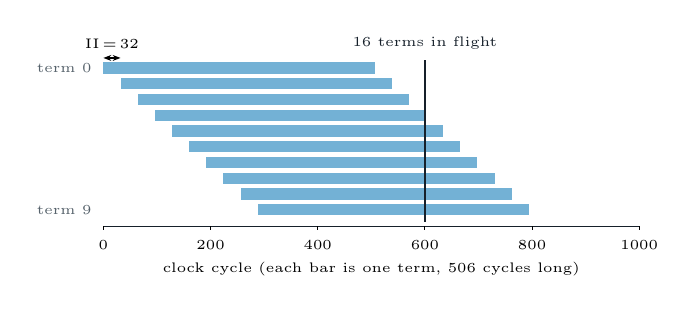
\begin{tikzpicture}[x=0.0068cm, y=0.2cm]
  \foreach \k in {0,...,9} {
    \pgfmathsetmacro{\s}{\k*32}
    \fill[acc!55] (\s, -\k) rectangle ++(506, 0.72);
  }
  \node[font=\tiny, text=muted, anchor=east] at (-4, 0.36) {term 0};
  \node[font=\tiny, text=muted, anchor=east] at (-4, -8.64) {term 9};
  \draw[ink, thick] (600,-9.4) -- (600,0.9) node[above, font=\tiny] {16 terms in flight};
  \draw[ink] (0,-9.7) -- (1000,-9.7);
  \foreach \c in {0,200,400,600,800,1000} { \draw (\c,-9.7) -- ++(0,-0.25) node[below, font=\tiny] {\c}; }
  \node[font=\tiny] at (500,-12.4) {clock cycle (each bar is one term, 506 cycles long)};
  \draw[{Stealth[length=1mm]}-{Stealth[length=1mm]}] (0,1.0) -- node[above, font=\tiny] {II\,=\,32} (32,1.0);
\end{tikzpicture}
\caption{Top: one COS term; the reverse sweep shares the forward datapath and reads forward values from scheduled rotating registers. Bottom: the modulo schedule (first 10 of 128 terms).}
\label{fig:sched}
\end{figure}

% =============================================================================
\section{Implementation and Methodology}
\label{sec:methodology}
\textbf{Configurations.} \texttt{z7} (56-bit, 8 multipliers, all on chip, 4,733 cycles);
\texttt{z7h} (the same with setup and finish on the host as bit-exact generated C, 128-term loop on
the FPGA, 4,572 cycles); \texttt{zu} (64-bit, 32 multipliers, all on chip, 1,593 cycles). Each sits
behind an AXI4-Lite register file, driven for testing by a JTAG-to-AXI master (Table~\ref{tab:impl}).

\textbf{Inputs.} A 21-case grid (moneyness, maturity, vol-of-vol, correlation; calls and puts); a
10,500-input sweep: 6,000 uniform over the domain ($S_0{=}100$, $K\in[60,150]$, $T\in[0.1,3]$,
$r\in[0,0.1]$, $v_0,\theta\in[0.005,0.25]$, $\kappa\in[0.2,6]$, $\xi\in[0.1,1]$, $\rho\in[-0.95,0.6]$),
500 in each of seven hard regimes (Feller violated, $\rho$ near its limits, deep strikes, short and long
maturities, high vol-of-vol, low variance) and 1,000 with one input outside; a held-out sweep of the
same composition drawn after the shift ranges were fitted; 50 board cases; and 50 calibrations to
NIFTY index options. Rounding error is measured against the same graph in double precision; the COS
result separately against a Fourier-integral price.

\textbf{Equal-throughput engines.} Price-only (4 multipliers), adjoint (8) and factored forward-mode
(10) \texttt{z7h}-style engines, II\,$=$\,32, generated, checked bit-exact against their models and
implemented out of context in Vivado 2025.2 (xc7z020clg484-1, 70\,MHz). The forward datapath carries
tangents without the per-term rescaling the adjoint applies, as a forward-mode AD tool would.

\textbf{CPU baselines.} The same algorithm in C++ (double, g++~13) on an Intel i5-1155G7 laptop
(4 cores): price only, bump-and-reprice, an optimised bump reusing the characteristic function,
forward-mode AD, taped adjoint AD (CoDiPack~\cite{codipack}) and hand-derived analytic
Greeks~\cite{cui}, \texttt{-O3 -march=native}; that build leaves the 128-term loop scalar, so a
structure-of-arrays variant split into seven loops over the terms is built with \texttt{-Ofast
-fopenmp-simd} and glibc's vector maths (a single-loop vectorised variant spills and is slower).
All match the reference (vectorised to $9.3\times10^{-12}$). Latency: best of five passes over 2,000
inputs on one idle core; throughput: eight processes. Table~\ref{tab:assumptions} lists the
assumptions.

\begin{table}[!t]
\centering
\caption{Board implementations (Vivado, post-route, JTAG systems)}
\label{tab:impl}
\footnotesize
\setlength{\tabcolsep}{2.4pt}
\begin{tabular}{@{}lccc@{}}
\toprule
& \textbf{ZedBoard} & \textbf{ZCU102} & \textbf{ZCU104}\\
\midrule
Device & xc7z020-1 & xczu9eg-2 & xczu7ev-2\\
Engine; cycles & \texttt{z7h}; 4,572 & \texttt{zu}; 1,593 & \texttt{zu}; 1,593\\
LUT & 38,752 (72.8\%) & 77,515 (28.3\%) & 77,863 (33.8\%)\\
FF & 32,134 (30.2\%) & 63,547 (11.6\%) & 63,796 (13.8\%)\\
DSP & 72 (32.7\%) & 510 (20.2\%) & 510 (29.5\%)\\
Clock (MHz) & 70 & 100 & 100\\
WNS (ns) & +0.458 & +1.601 & +1.469\\
On silicon & yes & yes & no\\
\bottomrule
\end{tabular}
\par\vspace{2pt}\parbox{\columnwidth}{\scriptsize Engine-alone $F_{\max}$ on the Zynq-7020 $\approx$79\,MHz (56-bit carry chains). Totals include the JTAG-to-AXI master and interconnect.}
\end{table}

\begin{table}[!t]
\centering
\caption{Assumptions, rationale and checks}
\label{tab:assumptions}
\scriptsize
\setlength{\tabcolsep}{2pt}
\begin{tabular}{@{}L{0.42cm}L{2.55cm}L{4.95cm}@{}}
\toprule
& \textbf{Assumption} & \textbf{Rationale; how checked}\\
\midrule
A1 & Bounded input domain & Shifters sized from measured ranges; held-out sweep: no in-domain flag, unflagged outside inputs within bound.\\
A2 & $S_0=100$ & Price homogeneous of degree one in $(S_0,K)$; host rescales.\\
A3 & $N{=}128$, range $c_1\pm10\sqrt{c_2}$ & Standard~\cite{fang}; method error measured separately (Sec.~\ref{sec:res-acc}).\\
A4 & $[a,b]$ fixed when differentiating & A numerical parameter; reference uses the same; Greeks within method error of a Fourier integral.\\
A5 & Calls by put--call parity & Call coefficients cancel in fixed point; worst call error 75$\times$ smaller.\\
A6 & First-order bound & Second-order terms $\approx2^{-FL}$ smaller; 50-digit check $\le$0.24 of bound; holds at 44 bits.\\
A7 & Local errors as in Sec.~\ref{sec:bound} & RTL bit-exact with the model; CORDIC errors measured.\\
A8 & 56/64-bit words & 56 bits: shortest with grid Greek error $\le1.2\times10^{-5}$; held-out tail weaker (Table~\ref{tab:acc}).\\
A9 & Latency = cycles $\times$ period & JTAG cannot time the engine; bus transfers (39 words) and \texttt{z7h} host steps excluded.\\
A10 & FPGA power from simulated activity & Routed netlist simulated on four bit-exact evaluations; vectorless 12.5\% underestimated dynamic power 3--6$\times$.\\
A11 & CPU package power (HWiNFO) & WSL cannot read it; idle 5.5\,W; power and throughput from the same run, Balanced plan, mains.\\
A12 & First-order Greeks; vega $=\partial V/\partial v_0$ & Gamma (second order) has a COS closed form~\cite{fang}; not built.\\
A13 & Hand-derived adjoint & Agrees with forward modes to $6\times10^{-14}$, CoDiPack to $1.3\times10^{-10}$.\\
A14 & NIFTY: calibrated, $r=0.06$ & Realistic test inputs, all in the domain.\\
\bottomrule
\end{tabular}
\end{table}

% =============================================================================
\section{Results}
\label{sec:results}
\subsection{Cost of the Greeks}
\label{sec:res-cost}
On the same hardware the price and nine Greeks take 1.04$\times$ the price alone on the 56-bit design
(4,733 vs.\ 4,568 cycles) and 1.55$\times$ on the 64-bit one, where the multipliers set the pace
(Fig.~\ref{fig:cycles}). These figures flatter the adjoint, since a price-only engine reaches the same II
with half the multipliers; at equal throughput the Greeks cost about 3\% in cycles on both designs
(4,733 vs.\ 4,613; 1,593 vs.\ 1,540). In Vivado (Table~\ref{tab:equal}) they cost 1.03$\times$ the
cycles, 1.68$\times$ the LUTs, 1.78$\times$ the flip-flops and 2$\times$ the DSP blocks of a right-sized
price-only engine (hand-derived Greeks cost 1.5 pricings in time on the CPU). Most of the 11,901
added flip-flops are the tape: 297 more rotating 56-bit registers than the price-only schedule, part of
which Vivado maps to shift-register LUTs. Bump-and-reprice takes 18.4$\times$ (56-bit) and 12.3$\times$
(64-bit) the adjoint's cycles on the same hardware; taking Delta and $\partial V/\partial K$ from the COS
sum and bumping only the other seven inputs (15 pricings) would be about 14.5$\times$ (estimated).

\begin{figure}[!t]
\centering
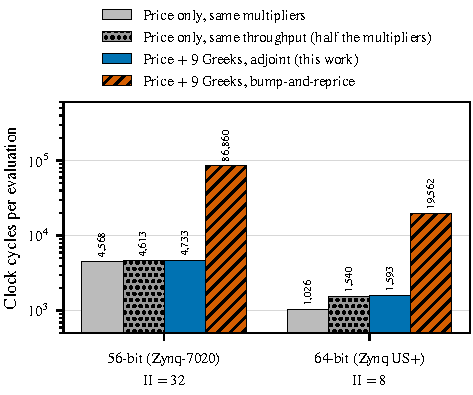
\includegraphics[width=\columnwidth]{figures/fig_cycles.pdf}
\caption{Cycles per evaluation (cycle-exact RTL simulation): price only on the same hardware and at the same II with half the multipliers, the adjoint engine, and bump-and-reprice.}
\label{fig:cycles}
\end{figure}

\begin{table}[!t]
\centering
\caption{Engines of equal throughput (II = 32), Zynq-7020, 70\,MHz}
\label{tab:equal}
\footnotesize
\setlength{\tabcolsep}{2.2pt}
\begin{tabular}{@{}lrrrrrr@{}}
\toprule
\textbf{Engine} & \textbf{Mult.} & \textbf{LUT} & \textbf{FF} & \textbf{DSP} & \textbf{Cycles} & \textbf{Worst err.}\\
\midrule
Price only & 4 & 21,251 & 15,303 & 36 & 4,457 & ---\\
\textbf{Adjoint} & \textbf{8} & \textbf{35,782} & \textbf{27,204} & \textbf{72} & 4,572 & $\mathbf{1.2\times10^{-5}}$\\
Fwd., factored & 10 & 38,199 & 30,514 & 90 & 4,449 & $7.4\times10^{-5}$\\
\bottomrule
\end{tabular}
\par\vspace{2pt}\parbox{\columnwidth}{\scriptsize Out of context, all bit-exact against their models (WNS $+0.377$, $+0.109$, $+0.275$\,ns). Worst err.: worst relative Greek error over the 21-case grid.}
\end{table}

\subsection{Adjoint against forward mode}
\label{sec:res-modes}
Three forward-mode datapaths were built by the same generator: \emph{dense} (all directions through
every operation, as a vector forward-mode tool; a weak baseline), \emph{sparse} (structural zeros
skipped) and \emph{factored} (exponent derivatives formed once per term, as a hand derivation of
analytic Greeks). All match the adjoint to $6\times10^{-14}$ in double precision. Per term the adjoint
needs 250 multiplications against 313, 396 and 802 (Table~\ref{tab:modes}); with 16 multipliers all but
the dense one are CORDIC-bound and the factored one is slightly faster. At equal throughput
(Table~\ref{tab:equal}) the factored engine is 2.7\% faster in cycles but needs 6.8\% more LUTs, 12.2\%
more flip-flops and 25\% more DSP blocks, and is 6$\times$ less accurate at the same word length because
its tangents are not rescaled. The adjoint's advantage over a well-factored forward datapath is real but
modest.

\begin{table}[!t]
\centering
\caption{Cycles by datapath and shared multipliers (scheduler)}
\label{tab:modes}
\footnotesize
\setlength{\tabcolsep}{3pt}
\begin{tabular}{@{}lrrrrr@{}}
\toprule
& & \multicolumn{2}{c}{\textbf{56-bit}} & \multicolumn{2}{c}{\textbf{64-bit}}\\
\cmidrule(lr){3-4}\cmidrule(l){5-6}
\textbf{Datapath} & \textbf{Mult./term} & \textbf{8} & \textbf{16} & \textbf{16} & \textbf{32}\\
\midrule
Price only & 126 & 4,566 & 4,561 & 1,538 & 1,024\\
\textbf{Adjoint} & \textbf{250} & \textbf{4,731} & 4,619 & \textbf{2,612} & \textbf{1,591}\\
Forward, factored & 313 & 5,622 & 4,571 & 3,069 & 1,795\\
Forward, sparse & 396 & 6,968 & 4,571 & 3,690 & 2,171\\
Forward, dense & 802 & 13,597 & 7,150 & 7,155 & 3,822\\
\bottomrule
\end{tabular}
\end{table}

\subsection{Accuracy and the bound}
\label{sec:res-acc}
\textbf{Rounding.} On the 21-case grid (Fig.~\ref{fig:accuracy}) the 56-bit price is accurate to
$6.1\times10^{-7}$ and the Greeks to at most $1.2\times10^{-5}$; the 64-bit design gains one to two orders
of magnitude; no output exceeds 0.103 of its bound. Over the 10,500-input sweep no unflagged result
exceeded its bound (worst 0.378) and nothing overflowed; on the held-out sweep no in-domain input was
flagged and the worst in-domain ratio was 0.356. In 50-digit arithmetic on 100 held-out inputs the error
is at most 0.24 of the bound, and the bound holds at 44 bits, where second-order terms are 4,096$\times$
larger (A6). The grid understates the tail (Table~\ref{tab:acc}): the price and market Greeks keep at
least 5.3 significant figures for 99\% of inputs, but $\partial V/\partial\kappa$ and
$\partial V/\partial\xi$ keep 3.5 and 3.0, and 2.2 and 1.4 at worst; for $\partial V/\partial\xi$ the bound
can exceed the value. Against bump-and-reprice on the same pricer (Fig.~\ref{fig:bump}) the adjoint is
32--560$\times$ more accurate (median 145$\times$) even with the best bump size chosen afterwards per Greek.

\textbf{COS method error.} The bound covers rounding only. Against a Fourier-integral price on the 50
board cases the method error has a median of $2\times10^{-11}$ for the price but reaches
$7.8\times10^{-3}$ for vega at $\xi=1$, $T=0.34$ (128 terms are too few; 256 remove it), far above the
bounded rounding error, and the engine does not flag it. A deployment would restrict the domain or use
$N=256$, roughly doubling the cycles.

\begin{figure*}[!t]
\centering
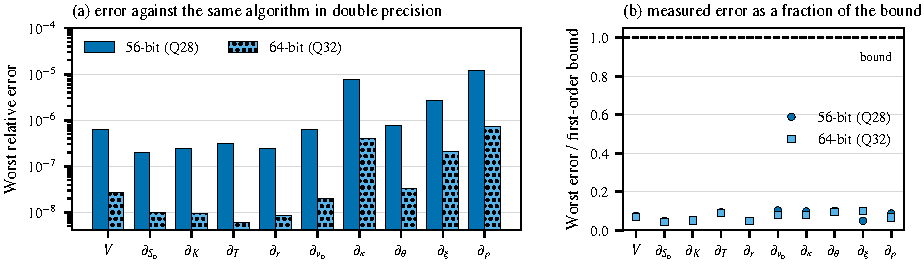
\includegraphics[width=\textwidth]{figures/fig_accuracy.pdf}
\caption{Rounding accuracy over the 21-case grid. (a) Worst relative error of the price $V$ and each Greek against the same graph in double precision. (b) Worst error divided by the bound (\ref{eq:bound}).}
\label{fig:accuracy}
\end{figure*}

\begin{figure*}[!t]
\centering
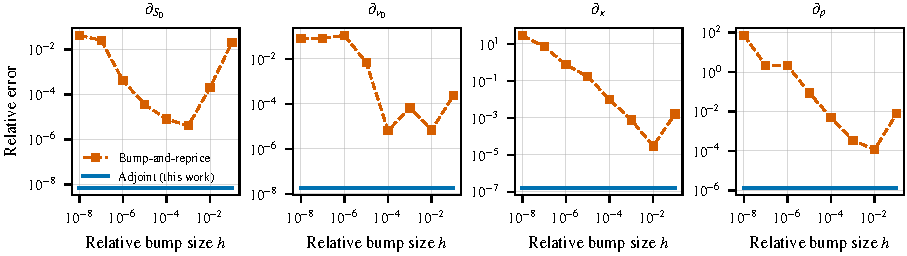
\includegraphics[width=\textwidth]{figures/fig_bump.pdf}
\caption{Relative error of bump-and-reprice against relative bump size, and of the adjoint engine, for four Greeks (56-bit design, base case); the other five behave alike.}
\label{fig:bump}
\end{figure*}

\begin{table}[!t]
\centering
\caption{Held-out sweep, 56-bit design, 9,500 in-domain inputs: significant figures and the bound relative to the value}
\label{tab:acc}
\footnotesize
\setlength{\tabcolsep}{3pt}
\begin{tabular}{@{}lccc|ccc@{}}
\toprule
& \multicolumn{3}{c|}{\textbf{Significant figures}} & \multicolumn{3}{c}{\textbf{$B_y/|y|$}}\\
\textbf{Output} & \textbf{Med.} & \textbf{P99} & \textbf{Worst} & \textbf{Med.} & \textbf{P99} & \textbf{Max}\\
\midrule
$V$ & 7.6 & 5.6 & 4.4 & 1e-6 & 6e-5 & 6e-4\\
$\partial_{S_0}$ & 8.1 & 5.7 & 3.9 & 3e-7 & 5e-5 & 3e-3\\
$\partial_{K}$ & 7.9 & 5.7 & 3.9 & 7e-7 & 6e-5 & 3e-3\\
$\partial_{T}$ & 7.6 & 5.5 & 4.0 & 1e-6 & 9e-5 & 3e-3\\
$\partial_{r}$ & 7.9 & 5.9 & 4.4 & 6e-7 & 4e-5 & 7e-4\\
$\partial_{v_0}$ & 7.6 & 5.3 & 3.3 & 8e-7 & 2e-4 & 4e-2\\
$\partial_{\kappa}$ & 6.0 & 3.5 & 2.2 & 3e-5 & 4e-3 & 7e-2\\
$\partial_{\theta}$ & 7.2 & 4.9 & 3.5 & 2e-6 & 3e-4 & 6e-3\\
$\partial_{\xi}$ & 5.9 & 3.0 & 1.4 & 4e-5 & 2e-2 & 1.1\\
$\partial_{\rho}$ & 7.0 & 4.9 & 3.7 & 4e-6 & 3e-4 & 6e-3\\
\bottomrule
\end{tabular}
\par\vspace{2pt}\parbox{\columnwidth}{\scriptsize Against the same graph in double precision; inputs where a Greek is within 1\% of zero excluded. A sample of the domain, not a supremum.}
\end{table}

\subsection{Silicon validation}
\label{sec:res-silicon}
Cases ran back to back with no reset (Table~\ref{tab:silicon}). Every output matched the bit-accurate
model, so the accuracy results and the bound hold on silicon; the worst error/bound ratio there was 0.255
and the worst 64-bit price error $7.3\times10^{-7}$.

\begin{table}[!t]
\centering
\caption{Silicon validation (outputs compared bit for bit with the model)}
\label{tab:silicon}
\footnotesize
\setlength{\tabcolsep}{2.5pt}
\begin{tabular}{@{}llrrc@{}}
\toprule
\textbf{Board} & \textbf{Inputs} & \textbf{Cases} & \textbf{Bit-exact} & \textbf{Err./bound}\\
\midrule
ZedBoard & vector + sweep & 1 + 50 & 459 / 459 & 0.199\\
ZCU102 & vector + sweep & 1 + 50 & 510 / 510 & 0.243\\
ZCU102 & NIFTY calibrations & 50 & 500 / 500 & 0.255\\
\midrule
\multicolumn{3}{@{}l}{\textbf{Total}} & \textbf{1,469 / 1,469} & $\le$\,0.255\\
\bottomrule
\end{tabular}
\par\vspace{2pt}\parbox{\columnwidth}{\scriptsize ZedBoard: 9 sums per case, finished on the host by bit-exact code; ZCU102: 10 outputs computed on chip. No \texttt{range\_err}.}
\end{table}

\subsection{Against a CPU}
\label{sec:res-cpu}
The FPGA latencies are computed (A9): they exclude the bus transfers and, for the ZedBoard, the host's
setup and finish; the CPU figures are measured whole evaluations (Fig.~\ref{fig:latency},
Table~\ref{tab:cpu}). The ZCU102 engine is 4.9$\times$ faster than forward-mode AD, 6.5$\times$ than taped
AAD, 15$\times$ than bump-and-reprice and 1.3$\times$ than scalar analytic Greeks, but one core running
the vectorised analytic Greeks (\SIMDUS\,$\mu$s) is 1.17$\times$ faster than the engine before its
transfers are counted, and four cores give \SIMDTP\ evaluations per second against 62,800 for one engine
(about 188,000 for the three that would fit on the ZCU102 by LUTs, not built). We claim no speed advantage.

\textbf{Energy}, counted at chip level on both sides: the FPGA device's on-chip power with the engine as
its only logic (dynamic from simulated activity, plus the device's static power), 0.676\,W and 2.485\,W,
gives 44 and 40\,$\mu$J per evaluation; the CPU package power (HWiNFO, A11) is 7.9 and 8.8\,W with eight
processes of the scalar and vectorised methods, giving 54.6 and 40.9\,$\mu$J (167 and 115\,$\mu$J on one
core). Neither includes DRAM or the board, and the FPGA excludes the host and bus. The 64-bit engine thus
matches the vectorised CPU and uses 1.4$\times$ less than the scalar build; counting only power above idle
(CPU, 15.4\,$\mu$J) against dynamic power (FPGA, 30\,$\mu$J), the CPU is ahead. We claim no energy advantage.

\begin{figure}[!t]
\centering
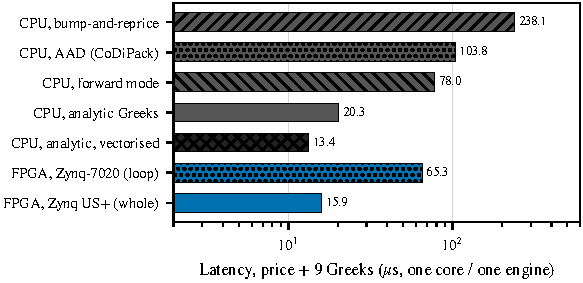
\includegraphics[width=\columnwidth]{figures/fig_latency.pdf}
\caption{Latency of one price and nine Greeks: one CPU core (i5-1155G7, idle; measured) and one FPGA engine (cycles $\times$ period, transfers excluded).}
\label{fig:latency}
\end{figure}

\begin{table}[!t]
\centering
\caption{Latency, throughput and energy per evaluation}
\label{tab:cpu}
\footnotesize
\setlength{\tabcolsep}{2.0pt}
\begin{tabular}{@{}lrrrr@{}}
\toprule
\textbf{Method} & \textbf{$\mu$s} & \textbf{Cost} & \textbf{Eval./s} & \textbf{Energy}\\
\midrule
CPU, price only & 13.7 & 1$\times$ & --- & ---\\
CPU, bump-and-reprice & 238.1 & 17.4$\times$ & --- & ---\\
CPU, optimised bump & 146.6 & 10.7$\times$ & --- & ---\\
CPU, adjoint (CoDiPack) & 103.8 & 7.6$\times$ & 26,900$^{a}$ & ---\\
CPU, forward mode & 78.0 & 5.7$\times$ & 34,000$^{a}$ & ---\\
CPU, analytic Greeks & 20.3 & 1.5$\times$ & 158,000$^{a}$ & 54.6\,$\mu$J$^{b}$\\
CPU, analytic, vectorised$^{e}$ & \SIMDUS & --- & \SIMDTP$^{a}$ & 40.9\,$\mu$J$^{b}$\\
\midrule
FPGA, ZedBoard, 70\,MHz (loop)$^{d}$ & 65.3 & 1.04$\times$ & 15,300 & 44\,$\mu$J$^{c}$\\
FPGA, ZCU102, 100\,MHz$^{d}$ & 15.9 & 1.55$\times$ & 62,800 & 40\,$\mu$J$^{c}$\\
\bottomrule
\end{tabular}
\par\vspace{2pt}\parbox{\columnwidth}{\scriptsize Cost: time relative to the price alone on the same platform and hardware. $^{a}$4 cores, 8 processes. $^{b}$Package power $\times$ run time / evaluations, 8 processes. $^{c}$Chip level, simulated activity (A10). $^{d}$Computed; transfers excluded. $^{e}$Structure of arrays, 29 Oct (scalar 22.7\,$\mu$s in the same session); throughput from the energy run.}
\end{table}

% =============================================================================
\section{Discussion and Conclusion}
\label{sec:discussion}
For a pricer without data-dependent control flow, a hand-derived reverse sweep can share one statically
scheduled datapath with the forward pass, its tape in scheduled registers. At equal throughput this costs
about 1.7$\times$ the area of a price-only engine at 1.03$\times$ its cycles, and is cheaper in multipliers
and logic, and more accurate at the same word length, than a well-factored forward-mode datapath built by
the same flow; each Greek has a first-order rounding bound that held on every input tested and on silicon,
on two FPGA families and on market calibrations. These are the claims. Speed and energy against a CPU are
not: a vectorised laptop core is faster, four cores give more throughput, and the energy per evaluation is
the same at chip level.

\textbf{Limitations.} The adjoint's advantage over a factored forward datapath is modest; Delta and
$\partial V/\partial K$ are nearly free in any COS implementation; the bound is a design-time tool that
excludes the COS method error, which dominates in a few in-domain cases; Gamma is not computed; latency
was computed, not measured, and board-level power is unmeasured; the Zynq-7020 design closes at 79\,MHz;
the domain is bounded. Strike chains, in which one reverse sweep per term serves every strike of an expiry
(32 strikes in 4,892 cycles, scheduled but not built), help a CPU as much (2.3\,$\mu$s per strike).
Deriving the reverse sweep automatically, adding Gamma, measuring end-to-end latency and board power, and
placing several engines per device are the next steps.

% =============================================================================
\begin{thebibliography}{99}
\bibitem{heston} S.~L. Heston, ``A closed-form solution for options with stochastic volatility with applications to bond and currency options,'' \emph{Rev. Financial Stud.}, vol.~6, no.~2, pp.~327--343, 1993.
\bibitem{fang} F.~Fang and C.~W. Oosterlee, ``A novel pricing method for European options based on Fourier-cosine series expansions,'' \emph{SIAM J. Sci. Comput.}, vol.~31, no.~2, pp.~826--848, 2008.
\bibitem{junike} G.~Junike, ``On the number of terms in the COS method for European option pricing,'' \emph{Numer. Math.}, 2024, doi:10.1007/s00211-024-01402-1.
\bibitem{albrecher} H.~Albrecher, P.~Mayer, W.~Schoutens, and J.~Tistaert, ``The little Heston trap,'' \emph{Wilmott Mag.}, pp.~83--92, Jan. 2007.
\bibitem{giles} M.~Giles and P.~Glasserman, ``Smoking adjoints: Fast Monte Carlo Greeks,'' \emph{Risk}, vol.~19, pp.~88--92, Jan. 2006.
\bibitem{capriotti} L.~Capriotti, ``Fast Greeks by algorithmic differentiation,'' \emph{J. Comput. Finance}, vol.~14, no.~3, pp.~3--35, 2011.
\bibitem{capgiles24} L.~Capriotti and M.~Giles, ``15 years of adjoint algorithmic differentiation (AAD) in finance,'' \emph{Quant. Finance}, vol.~24, no.~9, pp.~1353--1379, 2024.
\bibitem{griewank} A.~Griewank and A.~Walther, \emph{Evaluating Derivatives: Principles and Techniques of Algorithmic Differentiation}, 2nd~ed. Philadelphia, PA, USA: SIAM, 2008.
\bibitem{griewank92} A.~Griewank, ``Achieving logarithmic growth of temporal and spatial complexity in reverse automatic differentiation,'' \emph{Optim. Methods Softw.}, vol.~1, no.~1, pp.~35--54, 1992.
\bibitem{tapenade} L.~Hasco\"et and V.~Pascual, ``The Tapenade automatic differentiation tool: Principles, model, and specification,'' \emph{ACM Trans. Math. Softw.}, vol.~39, no.~3, 2013.
\bibitem{linnainmaa} S.~Linnainmaa, ``Taylor expansion of the accumulated rounding error,'' \emph{BIT Numer. Math.}, vol.~16, no.~2, pp.~146--160, 1976.
\bibitem{cui} Y.~Cui, S.~del~Ba\~no~Rollin, and G.~Germano, ``Full and fast calibration of the Heston stochastic volatility model,'' \emph{Eur. J. Oper. Res.}, vol.~263, no.~2, pp.~625--638, 2017.
\bibitem{codipack} M.~Sagebaum, T.~Albring, and N.~R. Gauger, ``High-performance derivative computations using CoDiPack,'' \emph{ACM Trans. Math. Softw.}, vol.~45, no.~4, 2019.
\bibitem{klai} M.~Klaisoongnoen, N.~Brown, and O.~Thomson~Brown, ``Low-power option Greeks: Efficiency-driven market risk analysis using FPGAs,'' in \emph{Proc. Int. Symp. Highly-Efficient Accelerators and Reconfigurable Technologies (HEART)}, 2022, pp.~95--101.
\bibitem{klaih2rc} M.~Klaisoongnoen, N.~Brown, and O.~Thomson~Brown, ``Fast and energy-efficient derivatives risk analysis: Streaming option Greeks on Xilinx and Intel FPGAs,'' in \emph{Proc. Int. Workshop Heterogeneous High-Performance Reconfigurable Computing (H2RC), SC22}, 2022.
\bibitem{klai24} M.~Klaisoongnoen, N.~Brown, T.~Dykes, J.~R. Jones, and U.-U. Haus, ``Evaluating Versal AI Engines for option price discovery in market risk analysis,'' in \emph{Proc. ACM/SIGDA Int. Symp. Field-Programmable Gate Arrays (FPGA)}, 2024.
\bibitem{deschryver} C.~de~Schryver \emph{et~al.}, ``An energy efficient FPGA accelerator for Monte Carlo option pricing with the Heston model,'' in \emph{Proc. Int. Conf. Reconfigurable Computing and FPGAs (ReConFig)}, 2011.
\bibitem{deschryver13} C.~de~Schryver, P.~Torruella, and N.~Wehn, ``A multi-level Monte Carlo FPGA accelerator for option pricing in the Heston model,'' in \emph{Proc. Design, Automation \& Test in Europe (DATE)}, 2013, pp.~248--253.
\bibitem{jin} Q.~Jin, D.~B. Thomas, W.~Luk, and B.~Cope, ``Exploring reconfigurable architectures for tree-based option pricing models,'' \emph{ACM Trans. Reconfigurable Technol. Syst.}, vol.~2, no.~4, art.~21, 2009.
\bibitem{tse} A.~H.~T. Tse, D.~Thomas, and W.~Luk, ``Design exploration of quadrature methods in option pricing,'' \emph{IEEE Trans. Very Large Scale Integr. (VLSI) Syst.}, vol.~20, no.~5, pp.~818--826, 2012.
\bibitem{vitisquant} AMD, ``Vitis Libraries: Quantitative Finance Library,'' [Online]. Available: \url{https://github.com/Xilinx/Vitis_Libraries}
\bibitem{zhang09} B.~Zhang and C.~W. Oosterlee, ``Option pricing with COS method on graphics processing units,'' in \emph{Proc. IEEE Int. Symp. Parallel \& Distributed Processing (IPDPS)}, 2009, pp.~1--8.
\bibitem{zhang14} B.~Zhang and C.~W. Oosterlee, ``Acceleration of option pricing technique on graphics processing units,'' \emph{Concurrency Computat.: Pract. Exper.}, vol.~26, no.~9, pp.~1626--1639, 2014.
\bibitem{gremse} F.~Gremse, A.~H\"ofter, L.~Razik, F.~Kiessling, and U.~Naumann, ``GPU-accelerated adjoint algorithmic differentiation,'' \emph{Comput. Phys. Commun.}, vol.~200, pp.~300--311, 2016.
\bibitem{gaffar} A.~A. Gaffar, O.~Mencer, W.~Luk, P.~Y.~K. Cheung, and N.~Shirazi, ``Floating-point bitwidth analysis via automatic differentiation,'' in \emph{Proc. IEEE Int. Conf. Field-Programmable Technology (FPT)}, 2002, pp.~158--165.
\bibitem{lee06} D.-U. Lee, A.~A. Gaffar, R.~C.~C. Cheung, O.~Mencer, W.~Luk, and G.~A. Constantinides, ``Accuracy-guaranteed bit-width optimization,'' \emph{IEEE Trans. Comput.-Aided Design Integr. Circuits Syst.}, vol.~25, no.~10, pp.~1990--2000, 2006.
\bibitem{gappa} F.~de~Dinechin, C.~Lauter, and G.~Melquiond, ``Certifying the floating-point implementation of an elementary function using Gappa,'' \emph{IEEE Trans. Comput.}, vol.~60, no.~2, pp.~242--253, 2011.
\bibitem{tang} P.~T.~P. Tang, ``Table-driven implementation of the exponential function in IEEE floating-point arithmetic,'' \emph{ACM Trans. Math. Softw.}, vol.~15, no.~2, pp.~144--157, 1989.
\bibitem{volder} J.~E. Volder, ``The CORDIC trigonometric computing technique,'' \emph{IRE Trans. Electron. Comput.}, vol.~EC-8, no.~3, pp.~330--334, 1959.
\bibitem{rau} B.~R. Rau, ``Iterative modulo scheduling: An algorithm for software pipelining loops,'' in \emph{Proc. 27th Annu. Int. Symp. Microarchitecture (MICRO)}, 1994, pp.~63--74.
\end{thebibliography}

\end{document}
